    \documentclass[15pt]{article}
\marginparwidth 0.5in 
\oddsidemargin 0.25in 
\evensidemargin 0.25in 
\marginparsep 0.25in
\topmargin 0.25in 
\textwidth 6in 
\textheight 8 in

\usepackage{graphicx}
\frenchspacing

\usepackage{amsmath}
\begin{document}
\vskip 1cm

\begin{figure}[htp]
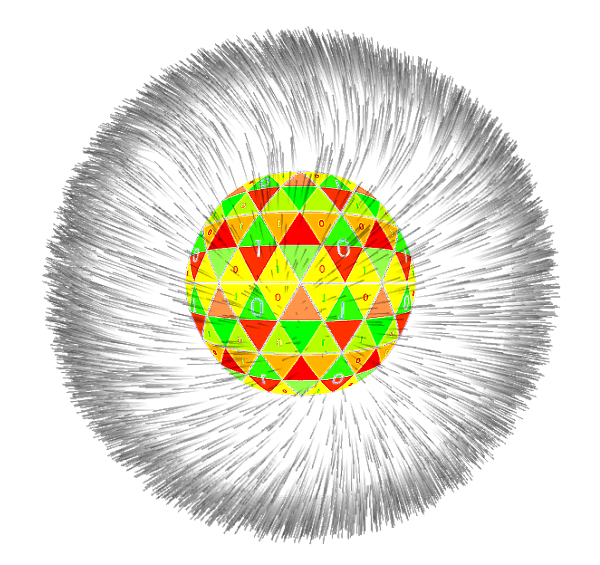
\includegraphics[scale=0.70]{./img/artee-1.png}
\caption{data-nodes arround a context domain space (mind's eye)}

\end{figure}


\title{\textbf{ACTIVE-MEMORY}}
\author{Hagen Geissler / santex\\
		C3D2}
\date{2012}


\maketitle



%-----------------------------------------------------------


\begin{center}


{\bf Short Description} \\[0.4cm]

\textbf{Procreating data}, under fitness consideration,
      in form of \textbf{semantic} micro-structures 
      within a conceptional domain.
      controlled by a human users request.
\vskip0.5cm


\begin{flushleft}


The projects goal is to establish a way to compound information quality  , quantity in a genetic fashion.

\vskip0.5cm

To organise knowledge like a biological organism. within a data population.

on data-nodes which are organisation,
in a context domain space.
Goal is to facilitate procreation in a genetic fashion. in essence to make better information from information.

Desired result of all efforts is to make better data from data by default.

It also has very interesting organisational properties,
each structure is bound on a concept or more.

Side effect of the genetic fitness evaluation
is that all root nodes and end nodes are known upfront reducing
query distance as each end-node is same distance.
It enables us to work kind of parallel.

\end{flushleft}




{\small New Terms } \\[0.1cm]
\textbf
{micro-structure}\\  
a micro-structure is a abstract entity describing 
\textbf{any concept}\\
the information is obtained via \textbf{WORD-NET}\\
\vskip0.4cm
\textbf
{key-stone}\\  
a key-stone is the root of a micro-structure 
\vskip0.4cm
\textbf
{example:}\\  
a micro-structure with the key-stone existence
\vskip0.2cm

\end{center}


          \begin{verbatim}
          <existence>
          - Cosmos
          - Unit
          - Universe
          - Physical_entity
          - Object
          - Physical_object
          - Nature
          - Macrocosm
          - Natural_order
          - World
          - Whole
          - Natural_object
          - Closed_universe
          - Existence
          - Creation
          - Entity
          \end{verbatim}


\vskip 1cm


\subsection{combining to a complex entity}
\begin{flushleft}	
\begin{figure}[htp]
\centering
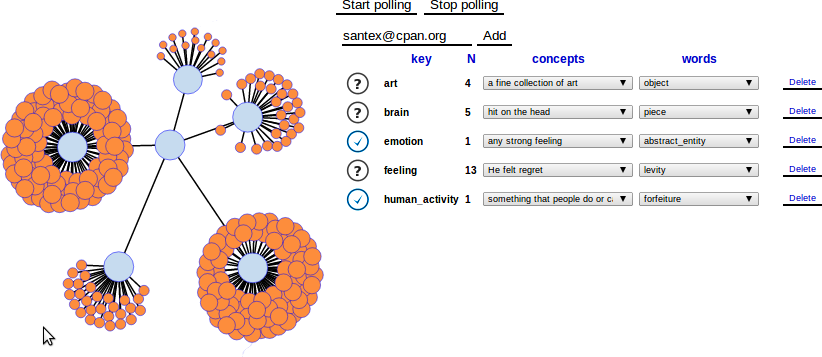
\includegraphics[scale=0.55]{./img/micro-structure-creation-implement.png}
\caption{making micro-structures}
\label{}
\end{figure}
\end{flushleft}
\begin{tabular}{lll}
	concept art & 4 sub-concepts & 27 key-words\\
	concept brain & 5 sub-concepts &  16 key-words\\
	concept emotion & 1 sub-concept &  28 key-words\\
	concept feeling & 13 sub-concepts &  76 key-words\\
	concept human-activity & 1 sub-concepts &  83 key-words\\

\end{tabular}
\vskip 1cm
	The core node is my user-name
\begin{flushleft}	
\begin{figure}[htp]
\centering
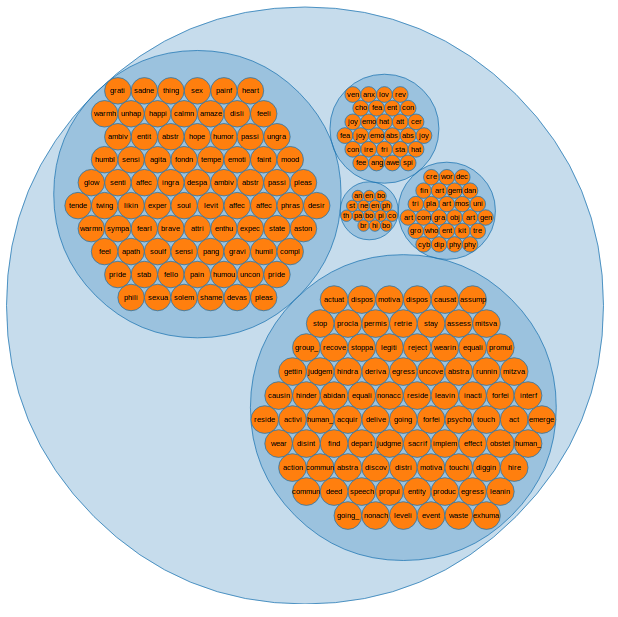
\includegraphics[scale=0.80]{./img/circle.png}
\caption{pack of concepts}
\end{figure}
\end{flushleft}
\vskip 5cm
\subsection{micro-structure properties}


\begin{itemize}
\item a micro-structure lives as a perl module (\$micro new existence)
\item most human concepts available
\item combine modular
\item access via terminal
\item micro-structure have access to the data-plug-in's (wiki, google, torrent)
\item the micro-structure is used as permanent query to scan for data.
\end{itemize}


\subsection{active-memory plug-ins}

\begin{itemize}
\item plug-ins are like feeds to just compatible to micro-structure's
\item currently in use wiki plug-in (google planed)
 

\end{itemize}



\vskip 2cm


\section{Fitness}  
  
Variables $\rightarrow$   

\begin{itemize}
\item C-total Word-net concept sum
\item C-established used concept sum
\item generation 
\item spawning links sum \textbf{in individual}
\item tag-number sum \textbf{in individual}
\item tag-ratios across total data population in micro-structure
\item tag-density across total data population in micro-structure
\item media items ratio \textbf{(links/amount media items)} (ogg, image, pdf)
\item special items ratio \textbf{(links/amount special items)} (category, list)
\item amount non linking/spawning individuals/
\end{itemize}

\vskip 0.4cm

\section{continuum of concepts within a micro-structure}  
  
\begin{itemize}
\item $\rightarrow$ \textbf{object}
\item natural object|physical object|celestial body|heavenly body
\item planet
\item outer planet
\item jovian planet
\item superior planet
\item major planet
\item gas giant
\item jupiter
\item Iapetus
\item moon
\item satellite
\item heavenly body|celestial body|physical object|natural object 
\item $\rightarrow$ \textbf{object};
\end{itemize}   
\vskip 9cm

\section{Project code structure}

\begin{itemize}
\item $\rightarrow$ \textbf{perl module}
\item $\rightarrow$ \textbf{memcache}
\item $\rightarrow$ \textbf{couchdb}
\item $\rightarrow$ \textbf{wordnet}
\end{itemize}   



\section{experimental Implementation}

\begin{itemize}
\item $\rightarrow$ \textbf{ui: http://www.quantup.com}
\item $\rightarrow$ \textbf{data-base: http://algoservice.com:5984/wikilist/}
\item $\rightarrow$ \textbf{git: https://github.com/santex/active-memory}
\end{itemize}   

\section{Network}
    
   \begin{tabular}{cc}
    Data in disorganised data network           &    The same network as micro-structure\\
    
    \end{tabular}




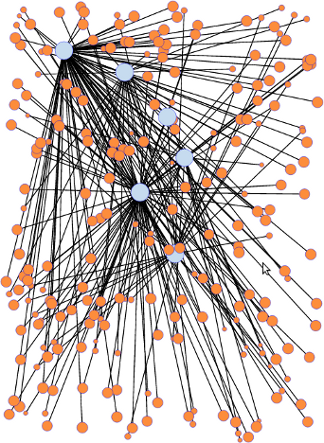
\includegraphics[scale=0.5]{img/normal-knowledge.png}
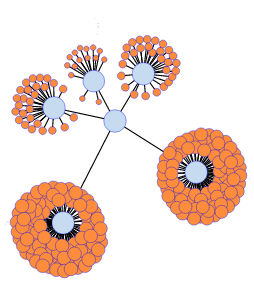
\includegraphics[scale=0.9]{img/micro-structure.png}


\vskip 0.4cm

    \begin{tabular}{cc}
    Data in disorganised data network           &|    The same network as micro-structure\\
    \\

    \end{tabular}

\section{A sample}

  \begin{verbatim}
hagen@sante12:~$ micro new hacker;
hagen@sante12:~$ micro hacker
physical_object
hagen@sante12:~$ micro hacker
person
hagen@sante12:~$ micro hacker
computer_user
hagen@sante12:~$ micro hacker
programmer
hagen@sante12:~$ micro hacker
someone
hagen@sante12:~$ micro hacker
organism
hagen@sante12:~$ micro hacker
engineer

now use > $ micro hacker 20
animate_thing
programmer
object
coder
computer_programmer
physical_object
living_thing
entity
software_engineer
physical_entity
engineer
cause
individual
applied_scientist
being
hacker
somebody
technologist
causal_agent
whole



  \end{verbatim}


\vskip 1cm


\section{A sample with data}


  \begin{verbatim}


   $ micro new constallation;
   $ micro constallation 103;
   
   
   
    andromeda
    antlia
    apus
    aquarius
    aquila
    ara
    argo
    aries
    auriga
    bootes
    caelum
    cancer
    canis_major
    canis_minor
    capricorn
    capricornus
    carina
    cassiopeia
    centaur
    centaurus
    cepheus
    cetus
    chamaeleon
    chameleon
    charioteer
    circinus
    columba
    coma_berenices
    constellation
    corona_borealis
    corvus
    crane
    crater
    crow
    crux
    crux_australis
    cygnus
    delphinus
    dorado
    dove
    draco
    dragon
    entity
    eridanus
    fornax
    gemini
    great_bear
    great_dog
    grus
    hercules
    hunter
    hydra
    hydrus
    indus
    leo
    lepus
    libra
    little_bear
    little_dog
    lupus
    lyra
    mensa
    microscopium
    musca
    natural_object
    norma
    object
    octans
    ophiuchus
    orion
    pavo
    pegasus
    perseus
    phoenix
    physical_entity
    physical_object
    pictor
    pisces
    puppis
    pyxis
    reticulum
    sagitta
    sagittarius
    scorpio
    scorpius
    sculptor
    serpens
    snake
    southern_cross
    southern_triangle
    taurus
    telescopium
    triangle
    triangulum
    triangulum_australe
    tucana
    unit
    ursa_major
    ursa_minor
    vela
    virgo
    volans
    vulpecula
\end{verbatim}
\vskip 1cm

get data this shell script only to balance load regular command 


(micro-wiki virgo)
.............................................................
\vskip 1cm

\begin{verbatim}
#!/bin/bash
IFS_BAK=$IFS;
IFS=$'\n';
array=( $(micro constallation 105) );
n=0;
for item in ${array[@]}
do
var=$(ps aux | grep -c perl);
if  [ 80 -lt $var ]; 
then 
  echo $n;
  sleep 10;
else
  micro-wiki $item &
fi
  let n+=1
done;
echo $n;
IFS=$IFS_BAK;
\end{verbatim}

\vskip 1cm

downloading\\
.............................................................\\

    
\begin{flushleft}
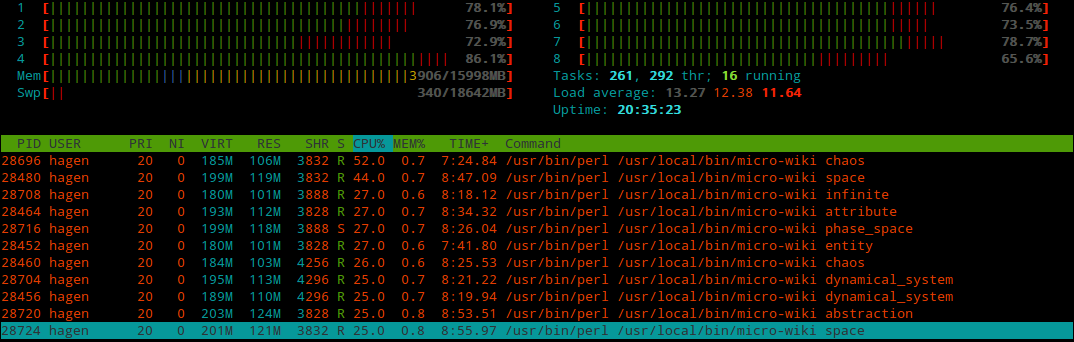
\includegraphics
[scale=0.43]{img/plugin.png}
\end{flushleft}
\vskip 1cm

sample out images (actually the image results are times 5)\\
.............................................................\\

    
\begin{flushleft}
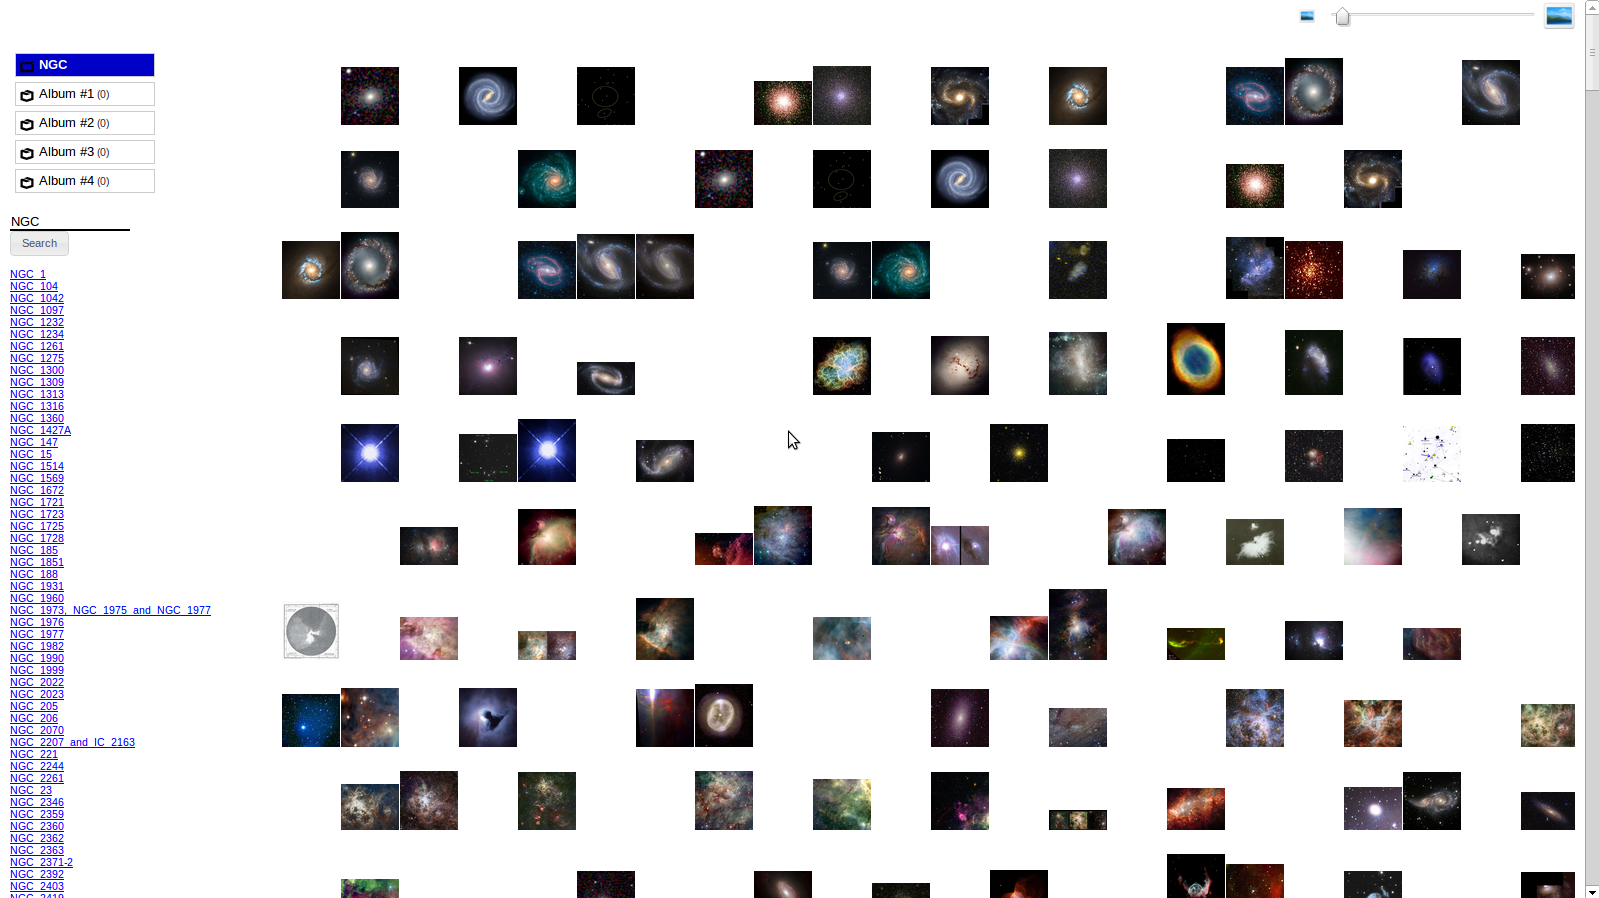
\includegraphics
[scale=0.29]{img/result-images.png}
\end{flushleft}
\vskip 5cm

\end{document}
  